\documentclass{article}

\usepackage{arxiv}
\usepackage[utf8]{inputenc} % allow utf-8 input
\usepackage[T1]{fontenc}    % use 8-bit T1 fonts
\usepackage{hyperref}       % hyperlinks
\usepackage{url}            % simple URL typesetting
\usepackage{booktabs}       % professional-quality tables
\usepackage{amsfonts}       % blackboard math symbols
\usepackage{nicefrac}       % compact symbols for 1/2, etc.
\usepackage{microtype}      % microtypography
\usepackage{amsmath}
\usepackage{lipsum}
\usepackage{caption}
\usepackage{float}

\newcommand{\der}[2][t]{\frac{\mathrm{d}#2}{\mathrm{d}#1}}

\title{Time Series Analysis of Chaotic Dynamical Systems with Recurrent Neural Networks}


\author{
  Lucas Wilson \\
  Undergraduate: Mathematics, Computer Science \\
  Colorado State University\\
  Fort Collins, CO 80523 \\
  \texttt{lkwilson96@gmail.com} \\
}

\begin{document}
\maketitle

\begin{abstract}
This is a paper about chaos.
\end{abstract}

%%% INTRODUCTION %%%
\section{Introduction}

This is a paper about chaos.
% TODO: mention \texttt{echonn}

%%% CHAOS %%%
\section{Chaos}

\subsection{History}

In 1963, Edward N. Lorenz published an article researching a simplified system of 
ordinary differential equations modeling a convective system \cite{lorenz1963deterministic}. His 
research popularized the possibility of a system being highly sensitive to 
initial conditions, i.e., chaos theory; while he wasn't the first to discover 
this phenomenon, he is considered to be the "official discoverer of chaos 
theory" \cite{oestreicher2007history}.

When forecasting, the goal is to have accurate predictions. However, 
a chaotic system's sensitivity to initial conditions implies that a small 
perturbation as a result of error will produce incorrect solutions.
Further, given a periodic
solution, we hope that a small perturbation, from error in measurement or from 
floating-point errors in numerical calculations, doesn't affect the solution or 
at least produces a quasi-periodic solution close to the periodic one. 
(A solution or trajectory $F$ 
is quasi-periodic if and only if for all $t$ and for some $\tau$, $F(t+\tau)$ 
is arbitrarily close to $F(t)$ \cite{lorenz1963deterministic}.)

An example of this is the trajectories of the sun and planets in our solar 
system. Newton's equations can be used to create a system of equations to model 
the bodies of mass (known as the n-body problem). However, with the existence of
other bodies of mass from other solar systems within the universe, we will have 
small perturbations introduced into the system. If the system is chaotic, then 
over time, the actual trajectories will diverge from our model's 
\cite{oestreicher2007history}. 

One of the defining characteristics of chaos is that the error from 
perturbations grows exponentially \cite{oestreicher2007history}. At the time of 
Lorenz's paper, unstable 
error was not well understood, and this led to Lorenz's surprising discovery 
\cite{oestreicher2007history}. Lorenz reported that a single iteration in 
calculating the solution to the dynamical system took 
approximately one second \cite{lorenz1963deterministic}. In his paper, he shows 
one of his calculations having about 3000 iterations, which must have taken 
around 50 minutes. Given the amount of time it takes to perform the calculation,
it's tempting to continue the calculation from the output of the previous 
calculation. However, the story of the discover is that while the computer used 
6 digit accuracy, it output only 3 digits, so when the simulation was continued 
by Lorenz with the less accurate measurements, he found the results to be very 
different \cite{oestreicher2007history}. 

Chaos can appear in many different situations. Lorenz's paper demonstrates chaos
in a dynamical system useful for forecasting convection in the atmosphere or 
liquids \cite{lorenz1963deterministic}. "Chaos theory has a few applications for
modeling endogenous biological rhythms such as heart rate, brain functioning, 
and biological docks" \cite{oestreicher2007history}. It can also appear in 
solutions to Hamiltonian problems such as the 3 body problem (as mentioned 
before) and the double pendulum problem (as I will show later). Understanding
the predictability of chaos is very useful to many different fields.

\subsection{Lyapunov Constant}

In terms of forecasting, it's useful to know how chaotic a dynamical system is. 
To measure this, we will measure the rate at which nearby trajectories 
diverge. Constants describing the divergence are known as the Lyapunov 
Characteristic Exponents (LCEs) \cite{sandri1996numerical}. There is an LCE for 
each dimension, and since they all represent exponential growth. The error 
growing at the rate of the largest LCE will dominate over the others.

% TODO: talk about attractors

Given a small perturbation $\epsilon$ to a dynamical system in the direction of 
the largest LCE, we can approximate the growth of the perturbation by the 
equation $\epsilon(\Delta t) = \epsilon_0 e^{\lambda \Delta t}$ where $\lambda$ 
is the largest LCE
\cite{bezruchko2010extracting}. For an LCE of zero, then the error doesn't grow
exponentially, and thus, there is no chaos. Error created
from smaller LCEs is negligible. The approximate time scale where 
perturbations become large is going to be proportional to $1 / \lambda$. This is
known as the Lyapunov time \cite{bezruchko2010extracting}. For our solar
system, the Lyapunov time is 10,000,000 years \cite{oestreicher2007history}.
Researchers have used it to evaluate the effectiveness of forecasting models on
chaotic problems \cite{pathak2018model}. Predicting the solution of
a chaotic model over an interval of time which is multiple times the size of the
Lyapunov time shows the predictability of a model.

In order to find the Lyapunov time, we only need to solve for the largest LCE. 
To find this, we will use a method detailed in \cite{viswanath1998lyapunov}.

% TODO: Lyapunov calculation

%%% DYNAMICAL SYSTEMS %%%
\section{Dynamical Systems}

Three dynamical systems will be used to demonstrate the predictability of 
chaotic systems: the Lorenz system, Poincaré's 3-body 
problem solution, and the double pendulum system.
The Poincaré system is the one of the first (possibly the first), and Lorenz
is a classical example. The double pendulum is commonly referred to as chaotic, 
and I will show this later.

\subsection{Lorenz System}

The Lorenz system was originally based on a system of equations modeling 
convection created by Saltzman \cite{lorenz1963deterministic} 
\cite{saltzman1962finite}. Simplified by Lorenz, it is defined as follows
\cite{lorenz1963deterministic}:

\begin{align}
    \der{x} &= \sigma (y - x), \nonumber \\
    \der{y} &= x (\rho - z) - y, \nonumber \\
    \der{z} &= x y - \beta z. \label{eq:lorenz_equation}
\end{align}

Not all parameters for the Lorenz equation will produce chaotic behavior. In 
Lorenz's article, he uses the parameter values $\sigma=10$, $\beta=8/3$, and
$\rho=28$ \cite{lorenz1963deterministic}, and it has a maximum LCE of $0.90566$ 
\cite{viswanath1998lyapunov}. There are other parameters which
produce chaotic results outlined in Table \ref{table:lorenz_params}. Also shown 
in Table \ref{table:lorenz_params} are the values calculated by my Python
module \texttt{echonn} are listed. These values are not as accurate, but 
demonstrate the sufficient accuracy of \texttt{echonn}.

\begin{table}[H]
    \centering
    \begin{tabular}{|l|l|l|l|l|l|l|}
         % TODO: \lambda_1?
         % TODO: calculated values
        \hline
        $\sigma$ & $\rho$ & $\beta$ & actual $\lambda$ & calculated $\lambda$ & relative error of calculated $\lambda$ \\
        \hline \hline
        16 & 45.92 & 4 & 1.50255 & & \\
        16 & 40 & 4 & 1.37446 & & \\
        10 & 28 & 8/3 & 0.90566 & & \\
        \hline
    \end{tabular}
    \caption{
        Lorenz Parameters and Largest Lyapunov Exponent
        \cite{viswanath1998lyapunov}
    }
    \label{table:lorenz_params}
\end{table}

\subsection{3-Body Problem}

\subsection{Double Pendulum}

The double pendulum is commonly cited to be chaotic 
\cite{stachowiak2006numerical} \cite{levien1993double}. Using the system 
of equations derived by Stachowiak \cite{stachowiak2006numerical}, the system is
defined as follows:

\begin{align}
    \der{\theta_1} &= \omega_1, \nonumber \\
    \der{\theta_2} &= \omega_2, \nonumber \\
    \der{\omega_1} &= 
    \frac{
        \sin(\theta_1 - \theta_2) \lbrack
            l_1 \cos(\theta_1 - \theta_2) \omega_1^2 + \omega_2^2
        \rbrack
    }{
        2 l_1 \lbrack
            1 + m_1 - \cos^2(\theta_1 - \theta_2)
        \rbrack
    }
    -
    \frac{
        (1 + 2 m_1) \sin \theta_1 + \sin(\theta_1 - 2 \theta_2)
    }{
        l_1 \lbrack
            1 + m_1 - \cos^2(\theta_1 - \theta_2)
        \rbrack
    }
    , \nonumber \\
    \der{\omega_2} &= \sin (\theta_1 - \theta_2) 
    \frac{
        (1+m_1) (\cos \theta_1 + l_1 \omega_1^2)
        +
        \cos(\theta_1 - \theta_2) \omega_2^2
    }{
        1 + m_1 - \cos^2(\theta_1 - \theta_2)
    }. \label{eq:doub_pen}
\end{align}

While the system is a Hamiltonian system, Stachowiak decided to define the first order 
derivative components as angular velocity as opposed to momentum. This won't affect
anything regarding the purpose of this paper.

Interestingly, the 
degree of chaos is dependent on the initial conditions \cite{levien1993double}. 
In the experiment, the initial conditions had angular velocities of zero, the outer 
pendulum was straight down, and the inner pendulum varied from 0 degrees to 180 degrees 
\cite{levien1993double}; the results showed that the LCE increased with theta. 

Repeating the same experiment, but with different parameters, the results are similar (see 
Figure \ref{fig:doub_pend_energy}).

\begin{figure}[H]
    \centering
    %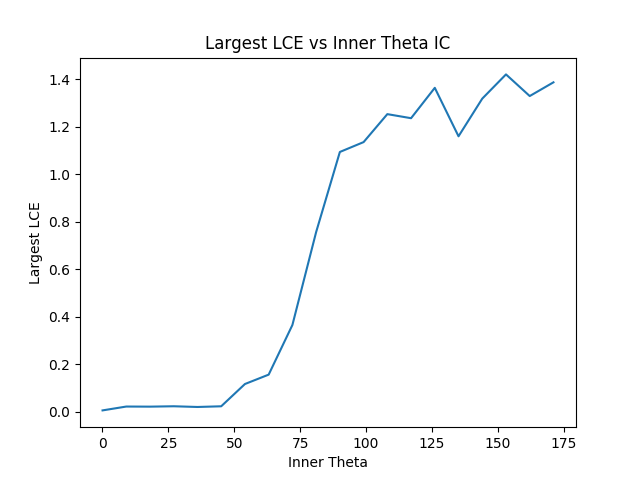
\includegraphics[.5\linewidth]{images/chaos_vs_energy_in_doub_pend.png}
    \caption{Largest Lyapunov Characteristic Exponent vs Inner Theta Initial Condition}
    \label{fig:doub_pend_energy}
\end{figure}



%%% MODELS %%%
\section{Models}

\subsection{ARIMA}
%\subsection{Recurrent Neural Networks}
\subsection{Echo State Networks}
%\subsection{LTSM}

%%% ANALYSIS %%%
\section{Analysis}

\subsection{Method}
\subsection{Results}

%% CONCLUSION %%%
\section{Conclusion}

\bibliography{references}
\bibliographystyle{unsrt}

\end{document}

% Useful LaTeX commands

%\section{Headings: first level}
%\subsection{Headings: second level}
%\subsubsection{Headings: third level}

%\keywords{First keyword \and Second keyword \and More}

% \paragraph{Paragraph}

%% \begin{figure}
%%   \centering
%%   \fbox{\rule[-.5cm]{4cm}{4cm} \rule[-.5cm]{4cm}{0cm}}
%%   \caption{Sample figure caption.}
%%   \label{fig:fig1}
%% \end{figure}

%%\author{
  %%Lucas Wilson \\
  %%Undergraduate: Mathematics, Computer Science \\
  %%Colorado State University\\
  %%Fort Collins, CO 80523 \\
  %%\texttt{lkwilson96@gmail.com} \\
  %% \AND
  %% Coauthor \\
  %% Affiliation \\
  %% Address \\
  %% \texttt{email} \\
  %% \And
  %% Coauthor \\
  %% Affiliation \\
  %% Address \\
  %% \texttt{email} \\
  %% \And
  %% Coauthor \\
  %% Affiliation \\
  %% Address \\
  %% \texttt{email} \\
%%}
